\documentclass[12pt,a4paper,oneside]{report}
\usepackage[T1]{fontenc}
\usepackage[utf8]{inputenc}
\usepackage{mathptmx}
\usepackage[left=30mm,right=23mm,top=24mm,bottom=24mm]{geometry}
\usepackage{graphicx,booktabs,longtable,array,tabularx,multirow}
\usepackage{amsmath}
\usepackage{setspace,enumitem,float,titlesec,fancyhdr}
\usepackage{tikz}
\usetikzlibrary{arrows.meta,positioning}
\usepackage{xurl}
\usepackage[hidelinks]{hyperref}
\usepackage{listings}
% Replace only the administrative fields below before institutional submission.
\newcommand{\ProjectTitle}{Kinematics, Workspace Estimation and Trajectory Planning of Six Robotic Manipulators Using ROS 2 and Gazebo}
\newcommand{\StudentName}{Vemula Kusumanjali}
\newcommand{\RegistrationNumber}{231801130015}
\newcommand{\GuideName}{Dr. N.V.S SHANKAR}
\newcommand{\GuideDesignation}{Associate Professor}
\newcommand{\Department}{Electronics and Communication Engineering}
\newcommand{\University}{Centurion University of Technology and Management}
\newcommand{\AcademicYear}{2026--2027}
\newcommand{\StudentORCID}{0009-0008-4421-5587}

\newcommand{\HODName}{K. JOGI NAIDU}
\newcommand{\DeanName}{Dr. SATYABRATHA LENKA}
\newcommand{\RegistrarName}{Prof. K.V. Ravi Kumar}
\newcommand{\ViceChancellorName}{P. Prasanta Umar Mohanty}

\hypersetup{pdftitle={\ProjectTitle},pdfauthor={\StudentName}}
\setstretch{1.25}
\setlength{\parskip}{5pt}
\setlength{\parindent}{0pt}\setlength{\emergencystretch}{3em}
\setlength{\headheight}{15pt}
\setlist{itemsep=2pt,topsep=4pt}
\titleformat{\chapter}[display]{\bfseries\Large\centering}{CHAPTER \thechapter}{8pt}{\Large}
\titlespacing*{\chapter}{0pt}{0pt}{18pt}
\titleformat{\section}{\large\bfseries}{\thesection}{.7em}{}
\titleformat{\subsection}{\normalsize\bfseries}{\thesubsection}{.6em}{}
\pagestyle{fancy}\fancyhf{}\fancyhead[L]{\small Six-Manipulator Robotics Laboratory}\fancyfoot[C]{\thepage}
\renewcommand{\headrulewidth}{.3pt}
\fancypagestyle{plain}{\fancyhf{}\fancyfoot[C]{\thepage}\renewcommand{\headrulewidth}{0pt}}
\lstset{basicstyle=\ttfamily\small,breaklines=true,columns=fullflexible,frame=single,showstringspaces=false}
\newcommand{\frontchapter}[1]{\chapter*{#1}\addcontentsline{toc}{chapter}{#1}}
\newcommand{\fig}[3]{\begin{figure}[H]\centering\includegraphics[width=#2\textwidth]{figures/#1}\caption{#3}\end{figure}}
\begin{document}
\begin{titlepage}\centering
{\Large\bfseries\ProjectTitle\par}\vspace{12mm}
A project report submitted in partial fulfilment of the requirements for the degree of\par\vspace{5mm}
{\large\bfseries BACHELOR OF TECHNOLOGY\par}\vspace{3mm}
in\par\vspace{3mm}
{\large\bfseries\Department\par}\vspace{10mm}
By\par\vspace{4mm}
{\large\bfseries\StudentName\par}\vspace{3mm}
Registration Number: \RegistrationNumber\par
Batch: 2023--2027\par
\small ORCID: \href{https://orcid.org/0009-0008-4421-5587}{\StudentORCID}\normalsize\par\vspace{10mm}
Under the guidance of\par\vspace{5mm}
\GuideName\par\vspace{3mm}\GuideDesignation\par\vfill

\includegraphics[height=29mm]{figures/university_logo.png}\par\vspace{4mm}
{\bfseries\University\par}
School of Engineering and Technology\par
Vizianagaram, Andhra Pradesh, India\par
Academic Year: \AcademicYear\par
\end{titlepage}
\pagenumbering{roman}
\thispagestyle{plain}
\addcontentsline{toc}{chapter}{BONAFIDE CERTIFICATE}
\begingroup
\definecolor{certificateblue}{RGB}{15,78,106}
\begin{center}{\Large\bfseries\color{certificateblue} BONAFIDE CERTIFICATE}\end{center}
\vspace{5mm}
Certified that this project report \textbf{\ProjectTitle} is the bonafide work of \textbf{``\StudentName\ (\RegistrationNumber)''} who carried out the project work under my supervision. This is to further certify to the best of my knowledge that this project has not been carried out earlier in this institute and the university.
\vspace{10mm}
\begin{flushright}
\begin{minipage}{.45\textwidth}\centering
SIGNATURE\\
\GuideName\\
\GuideDesignation
\end{minipage}
\end{flushright}
\vspace{14mm}
\textit{Certified that the above-mentioned project has been duly carried out as per the norms of the college and statutes of the university.}
\vspace{8mm}
\begin{flushright}
\begin{minipage}{.45\textwidth}\centering
SIGNATURE\\
\HODName\\
HOD (ECE)
\end{minipage}
\end{flushright}
\vfill
\begin{flushright}
\begin{minipage}{.50\textwidth}\centering
SIGNATURE\\[3mm]
\DeanName\\[3mm]
DEAN, SoET
\end{minipage}
\end{flushright}
\vspace{4mm}
\begin{center}
{\color{certificateblue}HEAD OF THE DEPARTMENT / DEAN OF THE SCHOOL}\\[2mm]
\textbf{Department of Electronics and Communication Engineering}\\
\textbf{DEPARTMENT SEAL}
\end{center}
\vspace{15mm}
\endgroup
\clearpage
\frontchapter{DECLARATION}
I, \StudentName, declare that this report entitled \textbf{\ProjectTitle} documents the educational robot models, software integration, numerical checks and recorded simulation results described in the report.

The report distinguishes calculated kinematic outputs from measured simulator feedback. It does not represent the educational geometries as calibrated commercial robots, and it does not present the proposed UR5e adaptive-workspace extension as completed experimental work. External software, technical references and supporting methods are acknowledged where used.

I will verify the institutional details and evidence accompanying this report before signing and submitting it for academic assessment.
\par\vspace{25mm}
Place: Vizianagaram\\[8mm]
Date: \underline{\hspace{4cm}}\hfill\rule{6cm}{.4pt}\\
\hspace*{.57\textwidth}\StudentName
\clearpage
\frontchapter{ACKNOWLEDGEMENT}
I express my sincere gratitude to my project guide, \textbf{\GuideName}, \GuideDesignation, for his guidance, feedback and encouragement throughout the development of this robotics project.

I thank \textbf{\HODName}, Head of the Department of Electronics and Communication Engineering, for the support extended during this project.

I express my sincere thanks to \textbf{\DeanName}, Dean of the School of Engineering and Technology, for the academic support and encouragement.

I am thankful to \textbf{\RegistrarName}, Registrar, and \textbf{\ViceChancellorName}, Vice Chancellor, \University, for providing an academic environment that supports learning and project work.

I also thank the faculty of the Department of Electronics and Communication Engineering and those who reviewed the demonstrations and helped refine the presentation of the project.

The development relied on the open-source ROS 2, RViz, Gazebo, Bullet, NumPy and SciPy ecosystems. Their documentation and software made it possible to connect mathematical robot models to interactive demonstrations and reproducible simulation analysis.

Finally, I thank my family and friends for their support throughout the implementation, testing and documentation of this project.
\par\vspace{12mm}\hfill\StudentName
\clearpage
\frontchapter{ABSTRACT}
This project develops a simulation-based laboratory for six robotic manipulators: SCARA, Stanford-type, PUMA-type, SCORBOT-type, Delta and Stewart platform. The objective is to connect forward and inverse kinematics, live parameter tables, sampled workspace estimation and smooth waypoint motion within a common ROS 2 interface. Four serial models use standard Denavit--Hartenberg transformations. Delta and Stewart mechanisms use geometry-based closed-loop constraints. The models are educational and are not calibrated replicas of commercial manipulators.

A Python graphical interface displays actuator values and tool poses, solves inverse-kinematics targets, samples workspaces and executes quintic actuator-space trajectories. RViz displays the calculated geometry. Dynamic verification is handled separately: serial mechanisms use articulated Gazebo models and joint controllers, while parallel mechanisms use a custom Gazebo System plugin containing native Bullet rigid-body dynamics. Recorded commands and simulator measurements are exported for analysis.

Retained numerical checks cover all six models. Four serial recordings excite joints J1 and J2, while two parallel recordings individually excite all three Delta actuators and all six Stewart legs. The parallel recordings contain 2,909 and 4,699 samples respectively. Maximum recorded constraint gaps are approximately 5.335 micrometres for Delta and 0.1908 micrometres for Stewart. All declared parallel screening gates pass for the prescribed small-motion trials. Serial results include transient tracking errors and nonzero gravity-related offsets, demonstrating why visual motion alone is insufficient to assess simulated control performance.

The principal outcome is an integrated educational platform with reproducible evidence and explicit validation boundaries. Collision-aware industrial task feasibility, hardware validation and adaptive UR5e workspace estimation remain future work.

\textbf{Keywords:} ROS 2; Gazebo; robot kinematics; serial manipulators; parallel manipulators; workspace; trajectory planning; simulation verification.
\clearpage
\tableofcontents
\clearpage\listoffigures
\clearpage\listoftables
\clearpage
\frontchapter{ABBREVIATIONS AND NOTATION}
\begin{tabularx}{\textwidth}{lX}
\toprule
Term & Meaning\\\midrule
ROS 2 & Robot Operating System 2; middleware and robotics tools\\
RViz & ROS visualisation tool\\
DOF & Degree of freedom\\
DH & Denavit--Hartenberg convention\\
FK / IK & Forward / inverse kinematics\\
URDF / SDF & Unified Robot Description Format / Simulation Description Format\\
PID & Proportional, integral and derivative control\\
CSV & Comma-separated values\\
WSL & Windows Subsystem for Linux\\
RMSE & Root-mean-square error\\
R / P & Revolute / prismatic joint\\
$\mathbf q$ & Actuator coordinates: radians or metres, according to joint type\\
$\mathbf p,R$ & Tool position vector and orientation matrix\\
$T$ & Homogeneous transform, or segment duration where stated\\
$q_d,q_m$ & Commanded and measured actuator coordinates\\
$e=q_m-q_d$ & Signed actuator tracking error\\
\bottomrule
\end{tabularx}

\clearpage\pagenumbering{arabic}
\chapter{INTRODUCTION}
\section{Background}
Robot manipulators combine mechanical geometry, coordinate transformations, control and software communication. Learning these topics separately can make it difficult to connect a joint value to an end-effector pose or to explain why a robot appears to move correctly but still has tracking error. A simulation laboratory provides an environment in which the learner can change an actuator coordinate, inspect the resulting transformation and observe an animated mechanism without requiring physical robot hardware.

ROS 2 supplies a modular communication framework for robotics applications \cite{ros2}. In this project it connects user input, visualisation and feedback monitoring. RViz presents geometric and state information, while Gazebo provides the environment for the separate dynamic demonstrations. A displayed pose and a dynamically achieved pose are treated as different kinds of output.

\section{Serial and parallel manipulators}
A serial manipulator consists of an open chain of joints and links. Its tool pose is obtained by composing successive link transformations. SCARA, Stanford-type, PUMA-type and SCORBOT-type models illustrate different joint arrangements and pose capabilities. A parallel manipulator connects the moving platform to the base through multiple branches; the branches must satisfy closure conditions simultaneously. Delta and Stewart models illustrate this second class.

Using both classes in one laboratory allows the same learning sequence to be repeated: inspect geometry, apply actuator inputs, calculate FK, request an IK solution, generate a trajectory and examine the resulting data. The mathematical method is selected for the mechanism rather than forcing every robot into a single open-chain representation.

\section{Project objectives}
\begin{enumerate}
\item Implement educational models of all six specified manipulators with explicit geometry, limits and units.
\item Display current actuator coordinates, serial DH parameters or parallel geometry, and tool position and orientation.
\item Provide FK, IK, sampled position workspaces and waypoint-based motion.
\item Integrate ROS 2 and RViz and provide separate Gazebo physics demonstrations.
\item Retain command/feedback recordings and evaluate tracking, closure and pose consistency within a clearly stated test scope.
\end{enumerate}
\section{Contribution and scope}
The project contribution is a common educational workflow and a verification package. It does not introduce a new general IK algorithm or establish superiority over existing robotics software. The recorded trials support the specific configurations, motions and settings used in those trials. They do not establish industrial accuracy, payload capability or collision-free operation.

This report follows the supplied college-report structure, expanding the methodology into robot modelling, implementation, experiments and results. The system uses an existing computer and software; no physical actuator wiring or fabricated hardware is part of the completed work.

\chapter{LITERATURE SURVEY}
\section{Robotics foundations}
Lynch and Park present rigid-body transformations, kinematics and motion planning in a common mathematical framework \cite{modern}. These concepts provide the basis for interpreting the pose of a serial end effector and for formulating closed-loop geometric constraints. This project applies established kinematic methods to educational robot geometries; the application and verification are the focus rather than a claim to new kinematics.

\section{ROS 2 and visualisation}
Macenski and co-authors describe the architecture and use of ROS 2 across robotics applications \cite{ros2}. Its communication model allows independent components to exchange state information. The laboratory uses this separation to keep the user interface, visualisation and recorded-feedback monitoring distinct. RViz is used to display robot markers and transforms \cite{rviz}; it is not treated as a rigid-body physics solver.

\section{Simulation and numerical solution tools}
Gazebo System plugins expose simulation lifecycle functions and support custom behaviour within the simulator \cite{gzplugin}. This enables the parallel add-on to integrate its dynamics with Gazebo visual entities. Bullet supplies the underlying rigid-body and constraint machinery \cite{bullet}. SciPy provides bounded nonlinear least-squares optimisation \cite{scipy}, used for numerical inverse kinematics and local closure reconstruction where appropriate.

\section{Workspace estimation and research extensions}
Gaussian-growth workspace sampling was proposed by Peidr\'{o} and colleagues to improve poorly sampled workspace regions \cite{gaussian}. Consequently, random point clouds and adaptive sampling alone should not be described as novel research contributions. The completed laboratory uses sampled workspaces for geometric interpretation. A separate proposal considers orientation, collision, approach clearance and manipulability for a UR5e assembly scenario; that proposal is discussed only as future work.

\begin{table}[H]\centering\small
\caption{Technical foundations and their use in this project}
\begin{tabularx}{\textwidth}{p{3.4cm}XX}\toprule
Source / method & Role in the project & Boundary of the claim\\\midrule
Rigid-body kinematics \cite{modern}&FK, IK and closure equations&Educational geometry, not vendor calibration\\
ROS 2 \cite{ros2}&Communication and modular integration&No middleware latency benchmark\\
RViz \cite{rviz}&Geometry and pose display&Rendering is not dynamic validation\\
Gazebo / Bullet \cite{gzplugin,bullet}&Recorded simulated response&Idealised bodies and disabled contact checks\\
SciPy least squares \cite{scipy}&Bounded numerical solution&Local solver success is not global completeness\\
Gaussian growth \cite{gaussian}&Context for future workspace research&Not implemented as a baseline in this report\\\bottomrule
\end{tabularx}
\end{table}
\section{Identified educational need}
A useful laboratory should expose the difference between a calculated pose, a visual representation and a measured simulation state. It should also retain test inputs and outputs so that a demonstration can be checked numerically. The present work addresses this educational integration need. A controlled student learning study has not been conducted, so improved learning outcomes are not claimed.

\chapter{PROBLEM STATEMENT AND REQUIREMENTS}
\section{Problem statement}
Develop a software laboratory for SCARA, Stanford, PUMA, SCORBOT, Delta and Stewart manipulators in which users can enter actuator coordinates or target poses, inspect the relevant model parameters, estimate reachable position regions and move through a sequence of points. The application must make the relationship between geometry and motion visible and provide separate evidence for simulated dynamic behaviour.

\section{Functional requirements}
\begin{table}[H]\centering\small
\caption{Functional requirements and implemented outputs}
\begin{tabularx}{\textwidth}{p{1cm}XX}\toprule
ID&Requirement&Output\\\midrule
F1&Select any of six models&Model-specific controls and geometry\\
F2&Apply actuator coordinates&Updated tool pose and rendered configuration\\
F3&Inspect robot parameters&DH table for serial chains; geometry tables for parallel models\\
F4&Solve a target pose&Accepted solution or solver failure message\\
F5&Estimate position workspace&Sampled point cloud within model limits\\
F6&Execute waypoints&Timed quintic actuator-space movement and path display\\
F7&Inspect simulated response&Command and measurement feedback from physics trials\\
F8&Retain numerical evidence&CSV recordings, summaries, plots and validation reports\\\bottomrule
\end{tabularx}
\end{table}
\section{Operating environment}
The user-side installation uses Windows with Ubuntu 24.04 under WSL 2, ROS 2 Jazzy and Gazebo Sim. The recorded parallel integration inventory identifies Gazebo Sim 8.15.0, Bullet 3.24, GCC 13.3 and CMake 3.28.3. Numerical validation also ran in a separate Linux environment; it must not be confused with the user's ROS/Gazebo runtime.

A display-capable computer and the relevant software packages are required. Processor model, installed memory and GPU performance were not retained as benchmark metadata, so this report makes no hardware-speed claim. The existing installation supports Python, NumPy, SciPy, Qt and the ROS 2 Python client library.

\section{Acceptance boundaries}
The project is assessed by observed functionality and retained evidence, not by a single completion percentage. Numerical checks establish model consistency over the tested cases. The four serial recordings cover J1/J2 excitation and holding of other coordinates. The two parallel trials cover individual small actuator excursions around home. Full-workspace dynamic coverage, physical hardware performance and all-joint serial excitation are outside the retained evidence.

\chapter{SYSTEM ARCHITECTURE AND METHODOLOGY}
\section{Three execution paths}
The architecture separates three paths. First, the kinematic path calculates robot geometry and sends markers to RViz; an optional Gazebo mirror displays the same calculated geometry. Second, the serial physics path creates articulated SDF models and uses Gazebo joint controllers. Third, the parallel physics path uses a custom Gazebo System plugin that owns a native Bullet dynamics world. Only the latter two paths provide recorded dynamic measurements.
\begin{figure}[H]\centering
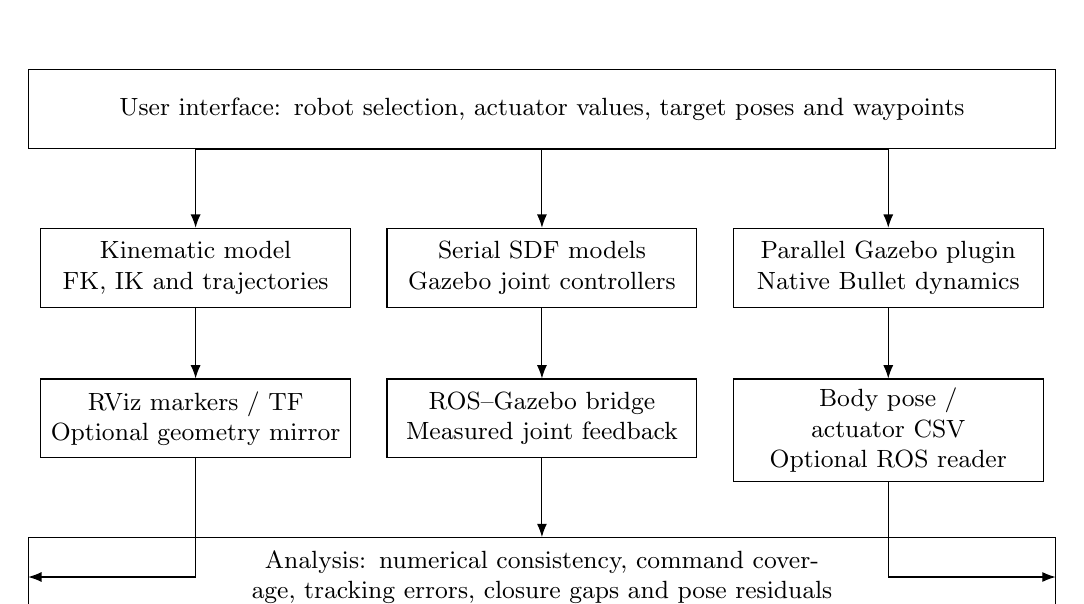
\begin{tikzpicture}[box/.style={draw,align=center,text width=3.7cm,minimum height=1.0cm,font=\small},>=Latex]
\node[box,text width=12.8cm] (u) {User interface: robot selection, actuator values, target poses and waypoints};
\node[box,below=1cm of u] (s) {Serial SDF models\\Gazebo joint controllers};
\node[box,left=.45cm of s] (k) {Kinematic model\\FK, IK and trajectories};
\node[box,right=.45cm of s] (p) {Parallel Gazebo plugin\\Native Bullet dynamics};
\node[box,below=.9cm of k] (v) {RViz markers / TF\\Optional geometry mirror};
\node[box,below=.9cm of s] (f) {ROS--Gazebo bridge\\Measured joint feedback};
\node[box,below=.9cm of p] (b) {Body pose / actuator CSV\\Optional ROS reader};
\node[box,text width=12.8cm,below=1cm of f] (a) {Analysis: numerical consistency, command coverage, tracking errors, closure gaps and pose residuals};
\draw[->](u.south)-|(k.north);\draw[->](u)--(s);\draw[->](u.south)-|(p.north);
\draw[->](k)--(v);\draw[->](s)--(f);\draw[->](p)--(b);
\draw[->](v.south)|-(a.west);\draw[->](f)--(a);\draw[->](b.south)|-(a.east);
\end{tikzpicture}
\caption{Software architecture. The visualisation and dynamic-feedback paths remain distinguishable.}
\end{figure}
\section{Software components}
\begin{table}[H]\centering\small
\caption{Main implementation components}
\begin{tabularx}{\textwidth}{p{4.1cm}X}\toprule
Component&Responsibility\\\midrule
\texttt{kinematics.py}&Robot definitions, transformations, IK and closure functions\\
\texttt{app.py}&Qt interaction, trajectory updates, tables and ROS outputs\\
\texttt{gazebo\_mirror.py}&Optional display of calculated geometry\\
\texttt{serial\_sdf.py}&Articulated serial model generation and coordinate mapping\\
\texttt{physics\_lab.py}&Serial simulation launch and command/feedback interface\\
\path{parallel_bullet_lab_v1}&Parallel dynamics core, Gazebo plugin and trial scripts\\
Analysis scripts&CSV statistics, pose consistency checks and plots\\\bottomrule
\end{tabularx}
\end{table}
\section{ROS interfaces and frames}
The consolidated interface publishes marker arrays on \texttt{/robot\_lab/markers}, actuator information on \texttt{/robot\_lab/joint\_states} and a transform from \texttt{world} to \texttt{lab\_tool}. Its marker-based display supports both serial and closed-loop mechanisms. The earlier SCARA demonstration used a robot-state-publisher/TF workflow; it should not be confused with the consolidated marker implementation.

Parallel feedback can be republished as joint states and a tool pose under \path{/parallel_lab/<robot>/}. These messages originate from the recorded simulator data. File-based republication supports monitoring and does not implement a hard-real-time controller.

\section{Working procedure}
\begin{enumerate}
\item Select a robot and load its geometry, actuator limits and home configuration.
\item Apply actuator values and compute FK, or solve IK for a requested target pose.
\item Update parameter tables and visual geometry from the accepted configuration.
\item Add waypoints and generate timed actuator-space segments.
\item Sample allowed configurations or poses to estimate the position workspace.
\item Run the separate physics trial when dynamic feedback is required.
\item Compare commands and measurements, retain CSV evidence and report the limits of each test.
\end{enumerate}


\chapter{ROBOT MODELLING AND KINEMATICS}
\section{Model families and units}
\begin{table}[H]\centering
\caption{Implemented educational manipulator structures}
\begin{tabularx}{\textwidth}{l l X}\toprule
Model&Actuated structure&Pose capability illustrated\\\midrule
SCARA&RRPR, 4&Translation and planar tool yaw\\
Stanford-type&RRPRRR, 6&Serial chain with a prismatic extension\\
PUMA-type&6R&Six-axis articulated serial motion\\
SCORBOT-type&5R&Five-axis arm with restricted pose capability\\
Delta&3R inputs&Translation with fixed platform orientation\\
Stewart&6P inputs&Platform translation and orientation\\\bottomrule
\end{tabularx}
\end{table}
Distances are stored in metres and rotations in radians. Degree-valued interface controls are converted at the boundary. The model names indicate educational structures. Their geometry and gains are not manufacturer specifications.
\section{Standard DH formulation}
For a serial link, the standard DH transform is
\begin{equation}
A_i=R_z(\theta_i)T_z(d_i)T_x(a_i)R_x(\alpha_i),\qquad {}^0T_n=\prod_{i=1}^{n}A_i.
\end{equation}
The corresponding homogeneous matrix is
\begin{equation}
A_i=\begin{bmatrix}
 c_\theta&-s_\theta c_\alpha&s_\theta s_\alpha&a_i c_\theta\\
 s_\theta&c_\theta c_\alpha&-c_\theta s_\alpha&a_i s_\theta\\
 0&s_\alpha&c_\alpha&d_i\\0&0&0&1
\end{bmatrix}.
\end{equation}
Here $c$ and $s$ denote cosine and sine. A revolute variable changes $\theta_i$; a prismatic variable changes $d_i$ with the model's specified sign. Multiplication order matters: rotations and translations generally do not commute.

\section{SCARA model and analytical checks}
The arm lengths are 0.30 m and 0.25 m. The consolidated model gives
\begin{align}
x&=0.30\cos q_1+0.25\cos(q_1+q_2),\\
y&=0.30\sin q_1+0.25\sin(q_1+q_2),\\
z&=0.235-q_3,\qquad \psi=q_1+q_2+q_4.
\end{align}
The negative sign in $z$ means that increasing the third coordinate lowers the tool. During the earlier TF demonstration, changing $q_3$ from 0.050 to 0.100 m changed tool height from 0.185 to 0.135 m. This checks the implemented coordinate convention.

For a target $(x,y,z,\psi)$, define
\begin{equation}
D=\frac{x^2+y^2-L_1^2-L_2^2}{2L_1L_2},\qquad q_2=\operatorname{atan2}(\pm\sqrt{1-D^2},D).
\end{equation}
Then
\begin{align}
q_1&=\operatorname{atan2}(y,x)-\operatorname{atan2}(L_2\sin q_2,L_1+L_2\cos q_2),\\
q_3&=0.235-z,\qquad q_4=\psi-q_1-q_2.
\end{align}
The two signs give candidate elbow configurations. Candidates must also satisfy actuator limits. The early test target $(0.30,0.20,0.15)$ m with zero yaw produced approximately $(-9.59^\circ,98.63^\circ,0.085\,\mathrm m,-89.04^\circ)$ and $(76.97^\circ,-98.63^\circ,0.085\,\mathrm m,21.66^\circ)$. These are two configurations for the same tool pose.

A target with $x=1$ m and $y=0.20$ m is outside the two-arm geometric reach because its planar radius exceeds $L_1+L_2=0.55$ m. Rejection of this target checks one clear infeasible case; it is not an exhaustive IK validation.

\section{Stanford, PUMA and SCORBOT models}
The Stanford-type model has a third prismatic coordinate with range 0.10--0.55 m. The PUMA-type model uses six revolute coordinates. The SCORBOT-type model uses five revolute coordinates and cannot generally achieve an arbitrary six-dimensional target pose. Their DH parameters are listed in Appendix~\ref{app:parameters} so the model is reproducible.

For a desired position $\mathbf p_d$ and orientation $R_d$, the consolidated serial solver minimises the bounded residual
\begin{equation}
\mathbf r(\mathbf q)=\begin{bmatrix}\mathbf p(\mathbf q)-\mathbf p_d\\\operatorname{Log}(R_d^TR(\mathbf q))^\vee\end{bmatrix}.
\end{equation}
The rotation-vector term describes orientation disagreement without directly subtracting Euler angles. The implementation uses the current configuration, home and six deterministic random seeds, with up to 250 function evaluations per solve. Acceptance uses $\|\mathbf r\|_2<10^{-5}$. Position and orientation residuals are unweighted metres and radians; this threshold is a numerical acceptance rule rather than a dimensionally homogeneous physical error.

Failure from these seeds means that the solver did not find a valid solution within its limits. It does not generally prove that no solution exists. Likewise, passing near-home tests does not prove correctness at every singular or boundary configuration.

\section{Delta closure model}
The educational Delta has base radius 0.28 m, platform radius 0.075 m, upper-arm length 0.20 m, lower-arm length 0.48 m and base height 0.85 m. For upper-arm endpoint $\mathbf e_i(q_i)$ and platform attachment offset $\mathbf a_i$, each lower branch imposes
\begin{equation}
\|\mathbf p+\mathbf a_i-\mathbf e_i(q_i)\|_2=0.48,\qquad i=1,2,3.
\end{equation}
Forward kinematics intersects the three equal-radius spheres and selects the lower assembly branch. Inverse kinematics obtains arm-angle candidates, checks limits and verifies consistency with the same branch. Platform orientation is fixed in this geometric model. A valid length equation alone is insufficient if a solution belongs to a different assembly branch.

\section{Stewart platform closure model}
The Stewart platform uses base radius 0.32 m and platform radius 0.20 m. Base anchor angles are $[10,110,130,230,250,350]^\circ$; platform angles are $[50,70,170,190,290,310]^\circ$. For platform pose $(\mathbf p,R)$, leg lengths follow
\begin{equation}
\ell_i=\|\mathbf p+R\mathbf a_i-\mathbf b_i\|_2,\qquad i=1,\ldots,6.
\end{equation}
The home pose is $(0,0,0.48)$ m with zero orientation. Leg lengths are limited to 0.30--0.75 m. Inverse kinematics directly evaluates the lengths. Forward kinematics numerically reconstructs a pose near the home or previous pose. It is a local closure solution, not a search over every possible assembly mode.

\chapter{WORKSPACE ESTIMATION AND TRAJECTORY PLANNING}
\section{Sampled position workspaces}
The geometric position workspace is the set of tool positions obtainable from allowable configurations. Finite sampling approximates this set. Retained exports contain 1,200 accepted points for each serial model and Delta, and 1,148 for Stewart. Serial models allow orientation to vary; the Stewart sampling uses a zero-orientation slice. The earlier SCARA demonstration used a denser 12,000-point display. These are different display/export settings, not contradictory measurements.

A sampled point cloud does not certify exact workspace volume. Uniform joint samples are generally nonuniform in Cartesian position, and empty regions can result from insufficient sampling. Collision checks are not included in these workspace plots. A position in the cloud is also not a guarantee that every desired orientation is achievable there.
\begin{figure}[H]\centering
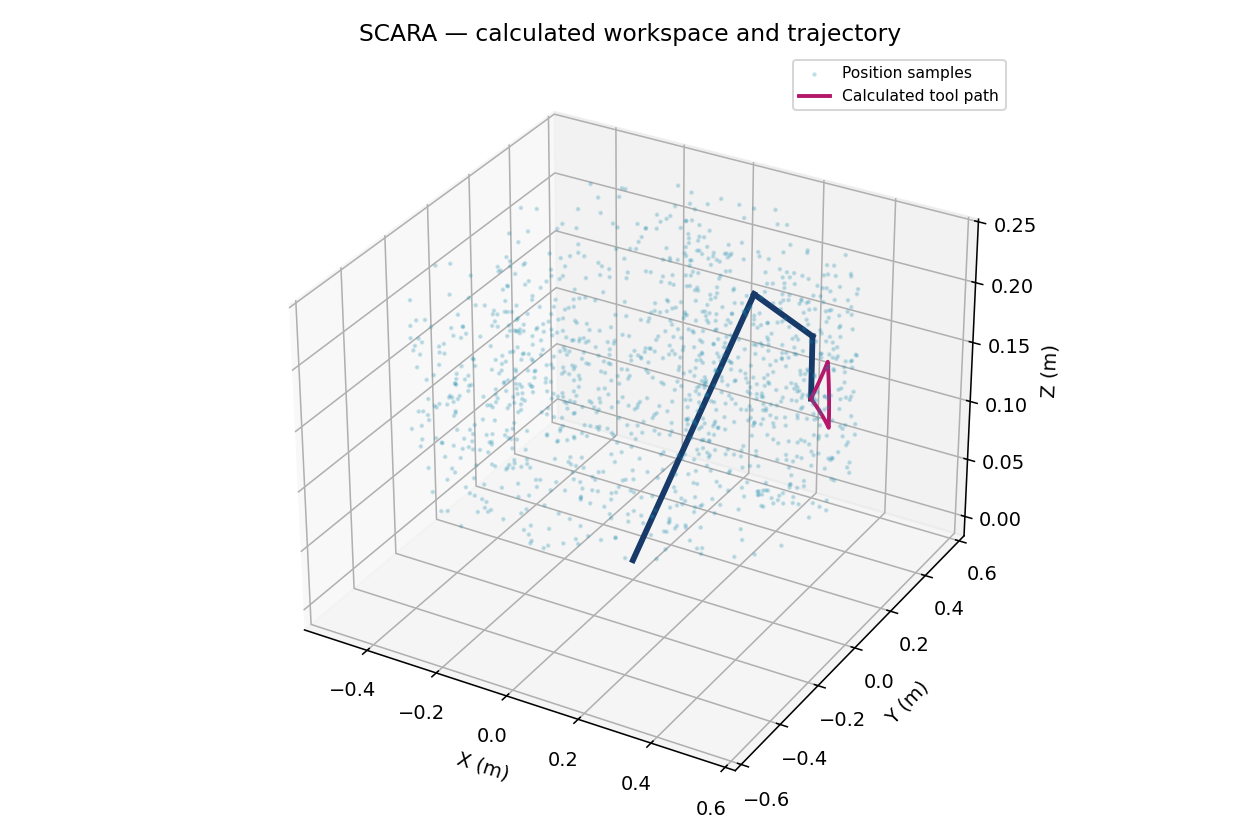
\includegraphics[width=.44\textwidth]{figures/SCARA_workspace.png}\hfill
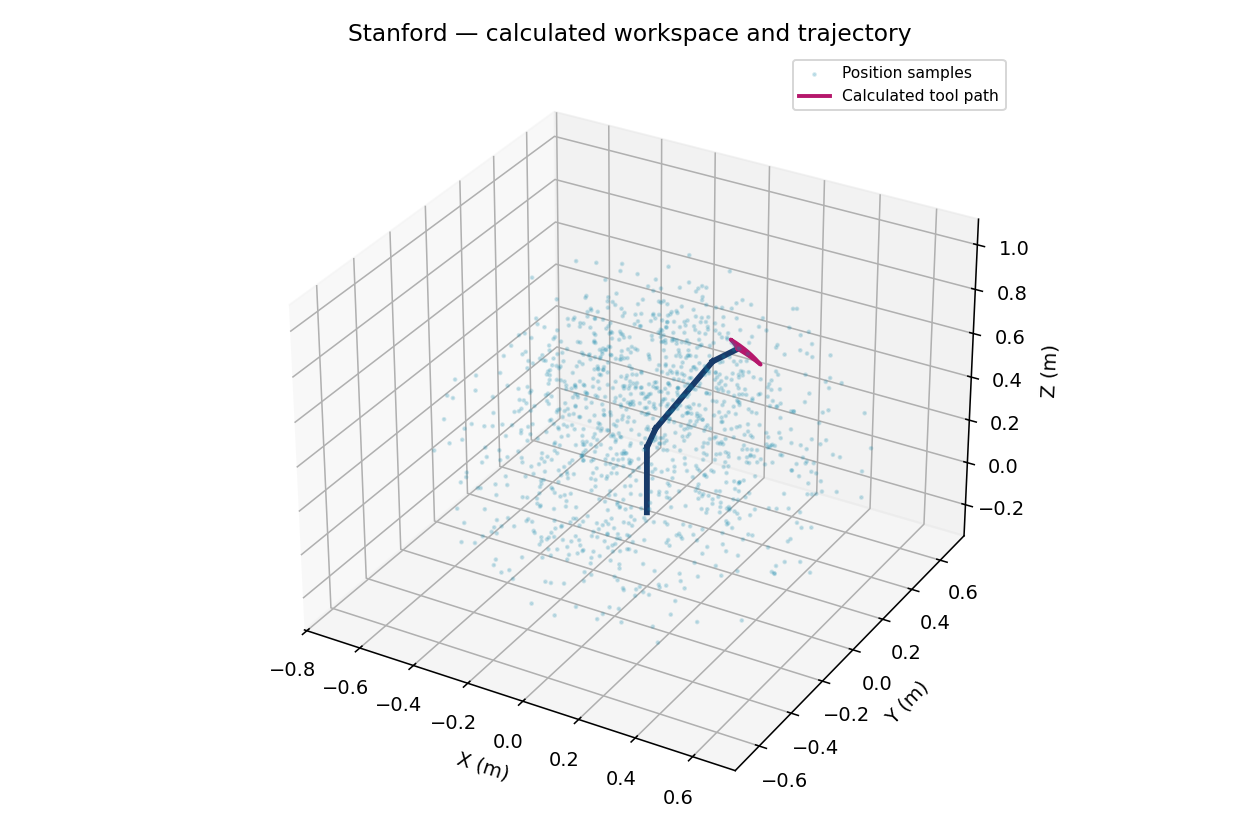
\includegraphics[width=.44\textwidth]{figures/Stanford_workspace.png}\\
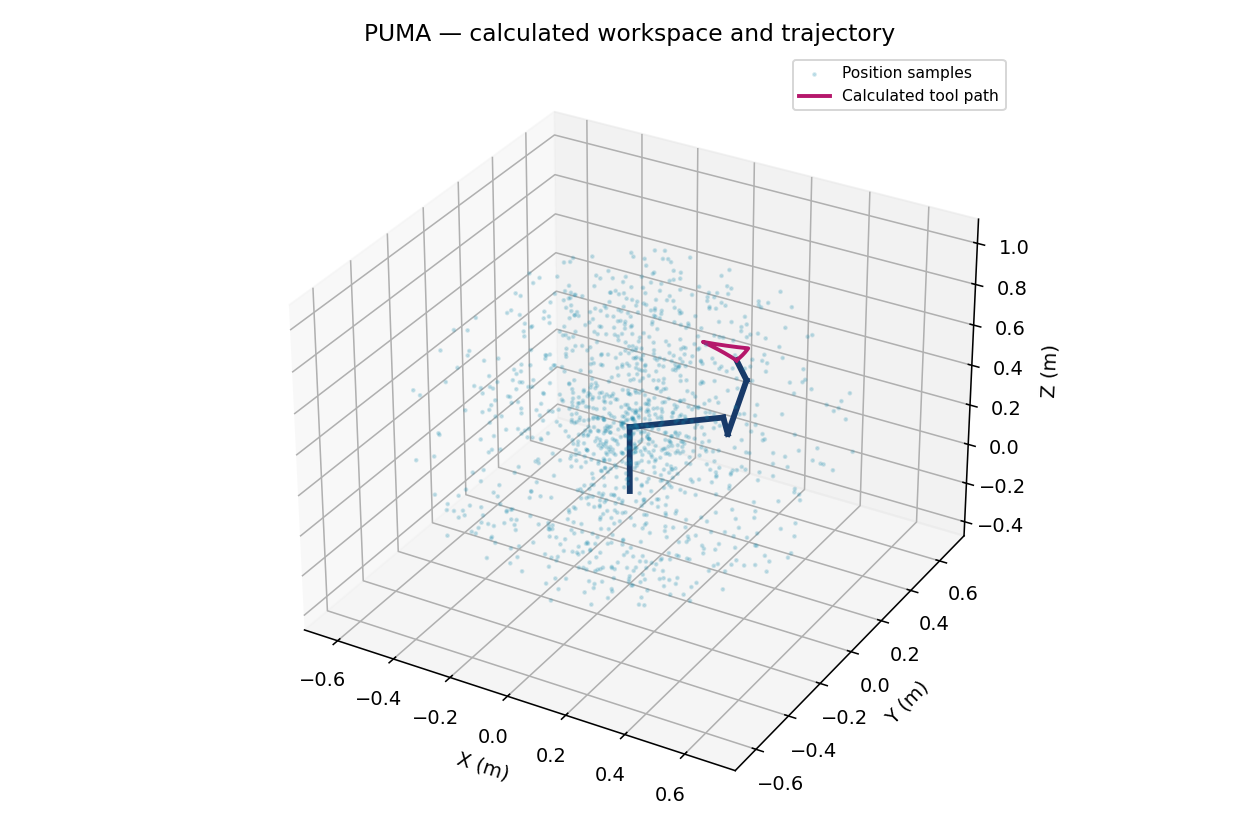
\includegraphics[width=.44\textwidth]{figures/PUMA_workspace.png}\hfill
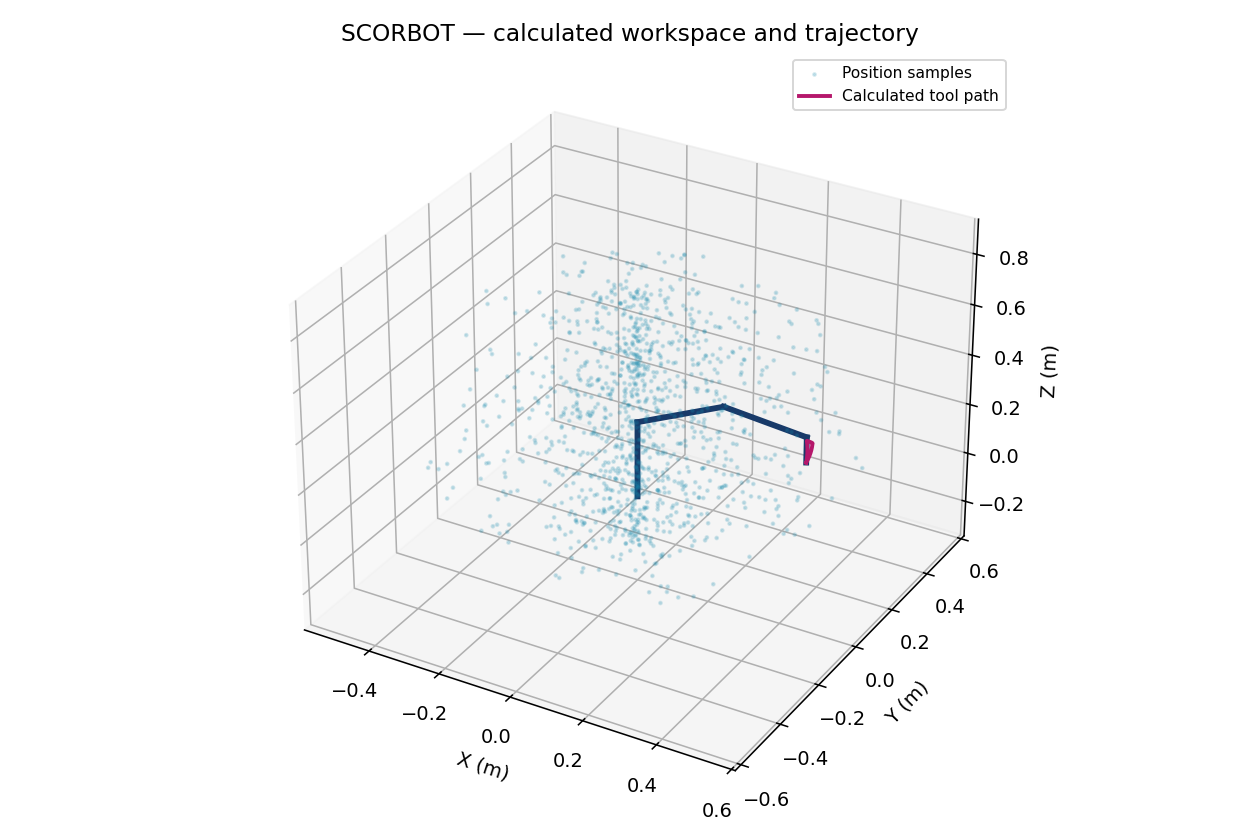
\includegraphics[width=.44\textwidth]{figures/SCORBOT_workspace.png}
\caption{Calculated position-workspace samples for the four serial educational models. These plots are model outputs, not physical measurements.}
\end{figure}
\begin{figure}[H]\centering
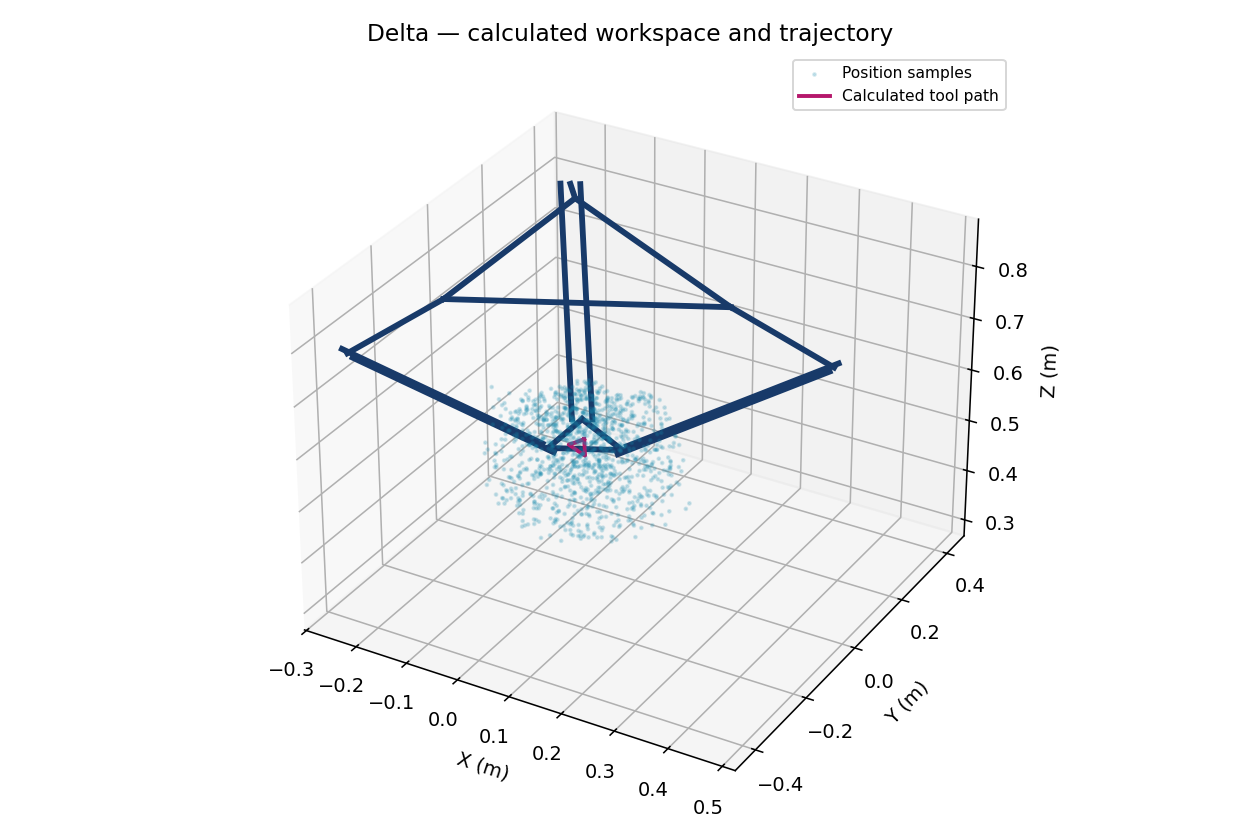
\includegraphics[width=.48\textwidth]{figures/Delta_workspace.png}\hfill
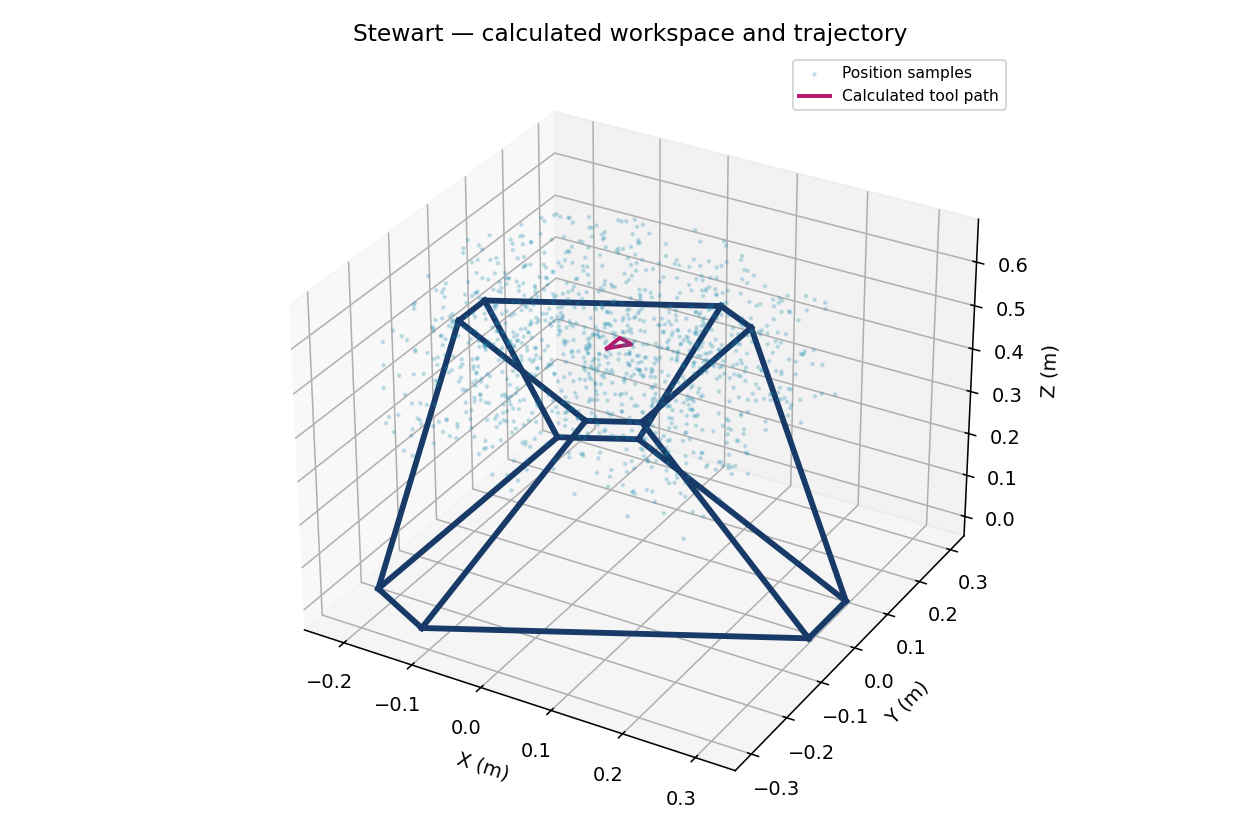
\includegraphics[width=.48\textwidth]{figures/Stewart_workspace.png}
\caption{Calculated parallel-model workspace samples. Delta has fixed platform orientation; Stewart illustrates a zero-orientation position slice.}
\end{figure}
\section{Quintic time scaling}
For actuator vectors $\mathbf q_a$ and $\mathbf q_b$, a segment of duration $T$ uses
\begin{equation}
\mathbf q(t)=\mathbf q_a+(\mathbf q_b-\mathbf q_a)s(u),\quad u=t/T,\quad s(u)=10u^3-15u^4+6u^5.
\end{equation}
This polynomial has zero velocity and acceleration at each end. All coordinates share the same normalised time, so they arrive together. The interpolation is in actuator space; a visually smooth end-effector path need not be a straight Cartesian line.

The maximum normalised speed is 1.875 and the maximum absolute normalised acceleration is approximately 5.774. Thus the duration is selected to satisfy
\begin{equation}
T\ge\max_i\left(T_{\rm requested},\frac{1.875|\Delta q_i|}{v_{i,\max}},\sqrt{\frac{5.774|\Delta q_i|}{a_{i,\max}}}\right).
\end{equation}
The educational limits are 0.8 rad/s and 1.6 rad/s$^2$ for revolute coordinates and 0.12 m/s and 0.25 m/s$^2$ for prismatic coordinates. These are implementation choices rather than actuator ratings.

\section{Waypoint execution and path checks}
The interface can load demonstration waypoints, add target waypoints, clear a sequence, run the sequence and export motion values. Each segment stops at its endpoint. Parallel closure is sampled along the proposed motion because valid endpoints alone do not establish a valid intermediate path. Discrete checking still cannot guarantee continuous feasibility or collision avoidance.



\chapter{GAZEBO DYNAMIC IMPLEMENTATION}
\section{Serial articulated models}
The serial SDF generator places links at the model's home configuration. Simulator coordinates are offset from model coordinates:
\begin{equation}
q_{\mathrm{gz},i}=q_i-q_{\mathrm{home},i}.
\end{equation}
Limits are shifted consistently, and feedback is converted back before comparison. Failing to apply this mapping would create apparent tracking errors even if the simulated joint were at its intended position.

The base is fixed. Nonzero-length links use cylindrical inertias and short links use spherical inertias. Gravity acts along negative $z$ at 9.81 m/s$^2$, the nominal simulation step is 1 ms and serial self-collision is disabled. Joint controllers use $(K_P,K_I,K_D)=(120,5,8)$ for revolute axes and $(600,5,30)$ for prismatic axes, with effort limits of $\pm100$ in the corresponding units.

ROS command topics follow \texttt{/physics\_lab/<robot>/cmd/joint\_<i>}. Serial tool positions in the feedback analysis are FK reconstructions from measured joints. They are not independent Cartesian sensor measurements.

\section{Native Bullet parallel plugin}
The parallel add-on owns a Bullet dynamics world inside a Gazebo System plugin. The standard Gazebo Physics system is omitted from these particular worlds so that two solvers do not update the same mechanism. The plugin steps the bodies and constraints, then copies the resulting body transforms to Gazebo entities for rendering.

This path is different from imposing FK poses in the optional geometry mirror. Mass, inertia, gravity, constraints and actuator forces/torques determine the simulated response. The Bullet solver uses 120 iterations and internal steps no larger than 1 ms. Contacts are disabled for the retained trials.

\begin{table}[H]\centering\small
\caption{Parallel dynamics model and controller settings}
\begin{tabularx}{\textwidth}{p{4.1cm}XX}\toprule
Parameter&Delta&Stewart\\\midrule
Actuation&3 hinge torques&6 axial leg forces\\
Moving platform mass&0.30 kg&1.00 kg\\
Branch body masses&Upper arm 0.20 kg; lower rod 0.06 kg&Each half-leg 0.15 kg\\
PID gains $(K_P,K_I,K_D)$&$(50,15,2.5)$&$(2500,600,60)$\\
Saturation&$\pm15$ N m&$\pm100$ N\\
Integral-state clamp&$[-0.2,0.2]$&$[-0.2,0.2]$\\
Contact model in trials&Disabled&Disabled\\\bottomrule
\end{tabularx}
\end{table}
\section{Mechanisms and feedback}
Delta uses three driven upper arms and six lower rods connected in paired branches. Stewart uses telescoping legs with point constraints at the base and platform and slider constraints between half-legs. Slider rotation is locked. This is an educational SPS-like realisation; universal-joint bearing-angle limits and calibrated actuator details are not represented.

The control law has proportional and integral position feedback with measured-velocity damping:
\begin{equation}
u_i=\operatorname{sat}\!\left[K_P(q_{d,i}-q_i)+K_I I_i-K_D\dot q_i\right].
\end{equation}
Delta receives hinge torque; Stewart receives equal-and-opposite axial forces on the two halves of each leg. Gains and masses are illustrative and require separate evaluation for other configurations or loads.

Actuator measurements are reconstructed from simulated body geometry. The platform pose is taken directly from the simulated platform body. Feedback is recorded at approximately 50 Hz with simulator timestamps; it includes commands, measurements, pose and the recorded constraint-gap diagnostic. The optional Python reader republishes these samples to ROS.

\chapter{EXPERIMENTAL PROCEDURE AND VERIFICATION}
\section{Evidence categories}
Three evidence categories are retained: numerical software checks, user-recorded visualisations and dynamic CSV recordings. They answer different questions. A screenshot establishes what was displayed; a numerical FK--IK round trip checks an implementation relationship; a simulator recording permits assessment of the simulated response under specified conditions.

The numerical validation report explicitly states that its script did not execute ROS or Gazebo. User-side physics recordings are the separate evidence for runtime trials. Combining the evidence requires preserving this distinction.

\section{Numerical validation}
The retained numerical suite checked each of the six models at home and at 12 near-home FK--IK round-trip cases. It also checked selected path closure, actuator timing and limits, generated SDF XML and rejection of a distant target. A separate serial-model suite checked articulated topology, positive inertia and agreement of the joint-coordinate mapping with DH at 80 random configurations per serial model.

These tests passed in the retained report. They establish consistency of the implemented educational models across those cases. They do not independently validate the geometry of a commercial robot or demonstrate global solver completeness.

\section{Serial trial protocol}
The four retained serial recordings vary J1 through 0.15 rad and J2 through 0.12 rad, returning to home. Other joint commands remain fixed. Different run lengths and holding intervals affect aggregate RMSE, so the four records are descriptive case studies rather than a controlled performance ranking.

The SCARA recording contains 5,131 samples including 63 duplicate simulation timestamps. All recorded rows are retained for sample-weighted statistics. The resulting RMSE is therefore not a time-integrated RMS over uniquely weighted timestamps.

\section{Parallel trial protocol}
After an initial 5 s hold, each parallel actuator is exercised individually for 12 s: 3 s outward motion, 3 s hold, 3 s return and 3 s at home. Excursions are 0.04 rad per Delta actuator and 0.004 m per Stewart leg. A final 10 s hold gives planned trial durations of 51 s and 87 s. Gazebo recordings continue to approximately 60 s and 96 s, respectively.

This protocol confirms individual actuator excitation near home. It does not exercise every combination of simultaneous actuator motion. Command spans are checked directly from the CSV data rather than inferred from animation.

\section{Error metrics and screening gates}
For sample $k$ and actuator $i$, define $e_i[k]=q_{m,i}[k]-q_{d,i}[k]$. The reported quantities are
\begin{align}
E_i^{\rm peak}&=\max_k|e_i[k]|,\\
E_i^{\rm final}&=|e_i[N]|,\\
E_i^{\rm tail}&=\max_{t_k\ge t_{\rm end}-5}|e_i[k]|,\\
\mathrm{RMSE}_i&=\sqrt{\frac{1}{N}\sum_{k=1}^{N}e_i[k]^2}.
\end{align}
Final-sample error and maximum error in the final five seconds are distinct. A small final value does not erase transient error earlier in the trial.

Every fifth parallel CSV sample is checked against independently implemented FK evaluated at the measured actuator coordinates. The residuals are
\begin{equation}
e_p=\|\mathbf p_{\rm body}-\mathbf p_{\rm FK}\|_2,\qquad e_R=\|\operatorname{Log}(R_{\rm FK}^{T}R_{\rm body})^\vee\|_2.
\end{equation}
The computational paths are separate, but they share nominal geometry; the comparison is not a physical measurement.

Parallel screening requires finite values, increasing timestamps, full trials, excitation of each actuator, measured limits within the checker's tolerance, recorded gap below 1 mm, sampled FK position residual below 1 mm and rotation residual below 0.01 rad. Tail tracking limits are 0.01 rad for Delta and 1 mm for Stewart. These are developer-selected investigation gates, not industrial acceptance specifications.

\chapter{RESULTS AND DISCUSSION}
\section{Six-model visual demonstration}
Figure~\ref{fig:six} presents the six manipulator families from user-recorded views. The SCARA panel comes from the earlier workspace demonstration; Stanford, PUMA and SCORBOT are shown in the consolidated RViz application; Delta and Stewart are shown in Gazebo. Different scales and configurations are used for readability.
\begin{figure}[H]\centering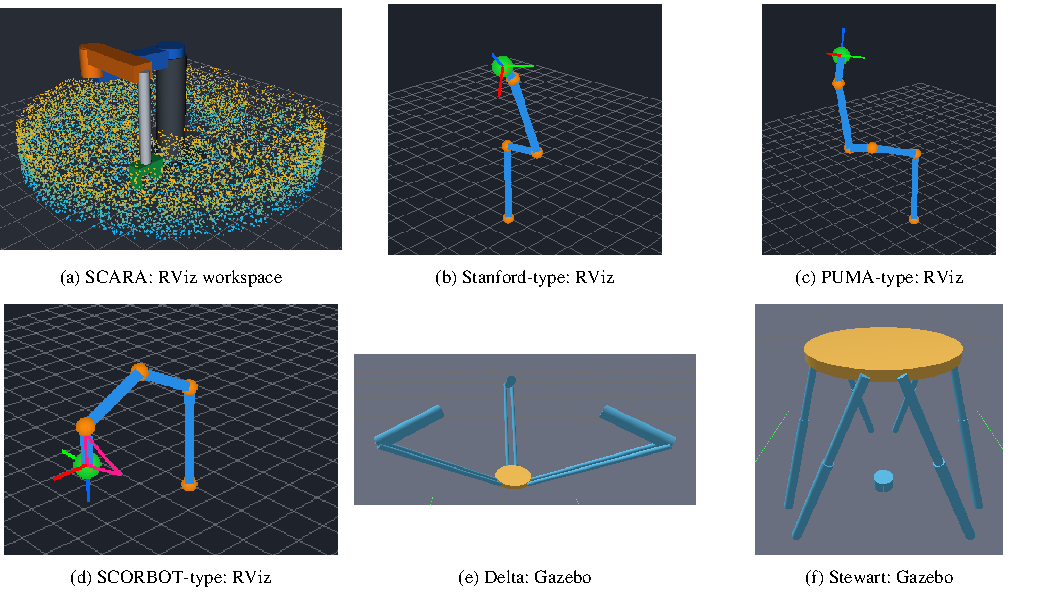
\includegraphics[width=\textwidth]{figures/six_robot_overview.pdf}
\caption{Six educational manipulators in recorded displays. The images establish rendering and are not accuracy measurements.}\label{fig:six}
\end{figure}
\section{Serial recorded results}
\begin{table}[H]\centering\small
\caption{Serial recordings and excited-joint RMSE}
\begin{tabular}{lrrrr}\toprule
Model&Samples&Time range (s)&J1 RMSE ($^\circ$)&J2 RMSE ($^\circ$)\\\midrule
SCARA&5131&0.068--255.272&0.09166&0.08957\\
Stanford&4683&0.068--223.278&0.28340&0.26880\\
PUMA&3258&0.068--157.862&0.31114&0.65648\\
SCORBOT&5169&0.986--249.798&0.16837&0.37221\\\bottomrule
\end{tabular}
\end{table}
\begin{table}[H]\centering\small
\caption{Peak and final absolute serial tracking errors for excited joints}
\begin{tabular}{lrrrr}\toprule
Model&J1 peak ($^\circ$)&J2 peak ($^\circ$)&J1 final ($^\circ$)&J2 final ($^\circ$)\\\midrule
SCARA&1.42381&1.22554&0.0000355&0.004048\\
Stanford&2.45232&2.19068&0.000146&0.000206\\
PUMA&2.39784&2.71810&0.000566&0.005526\\
SCORBOT&2.02604&2.53900&0.0000115&0.003381\\\bottomrule
\end{tabular}
\end{table}
The traces show transient deviations when commands change, followed by smaller errors during holding. All four records exhibit the intended J1/J2 command spans. Different geometries, gains, units and hold durations prevent these statistics from supporting a general ranking of the robots.
\fig{serial_errors.pdf}{1}{Measured-minus-commanded J1 and J2 angles in the four serial recordings.}
Held coordinates also matter. Final absolute prismatic J3 errors are approximately 0.916 mm for SCARA and 2.107 mm for Stanford. A stationary command therefore does not imply zero position error in a gravity-loaded simulation. No universal pass/fail threshold for serial tracking was declared for these original recordings.

The recordings predate later launcher timing changes. They document the runtime that produced them and should not be interpreted as regression coverage for every subsequent code change.

\section{Parallel recorded results}
\begin{table}[H]\centering\small
\caption{Parallel Gazebo trial statistics; maxima are across actuators where applicable}
\begin{tabularx}{\textwidth}{Xrr}\toprule
Metric&Delta&Stewart\\\midrule
Recorded samples&2909&4699\\
Final simulator time (s)&59.998&95.988\\
Excursion per actuator&0.04 rad&4 mm\\
Peak absolute actuator error&0.01414 rad&1.3359 mm\\
Final-five-second maximum error&$2.1935\times10^{-6}$ rad&$6.557\times10^{-4}$ mm\\
Maximum recorded constraint gap ($\mu$m)&5.335&0.1908\\
Sampled FK position residual ($\mu$m)&5.924&0.2446\\
Sampled FK orientation residual (rad)&$1.110\times10^{-4}$&$5.941\times10^{-7}$\\
Declared investigation gates&Passed&Passed\\\bottomrule
\end{tabularx}
\end{table}
Every Delta input and every Stewart leg has a nonzero command span in its recording. Early transients are larger than the final-five-second errors. The displayed traces are therefore necessary to interpret the small tail values in context.
\fig{parallel_tracking.pdf}{1}{Parallel actuator offsets, tracking errors and recorded closure diagnostics. Commands are dashed and measurements are solid in the top row.}
The constraint-gap and FK residual values are numerical consistency results in idealised simulations. Their micrometre-scale magnitudes do not establish micrometre physical positioning accuracy. They are also not a basis for claiming Stewart is intrinsically more accurate than Delta, because mechanisms, units, geometry and controller settings differ.

\section{Outcome against objectives}
\begin{table}[H]\centering\small
\caption{Evidence-supported project outcomes}
\begin{tabularx}{\textwidth}{p{4cm}X}\toprule
Objective&Retained evidence and interpretation\\\midrule
Six-model kinematics&Near-home numerical checks pass for all six educational models\\
Interactive visualisation&User-recorded views and confirmed moving demonstrations\\
Workspace estimation&Calculated sampled position clouds; no volume certificate\\
Waypoint movement&Quintic timing implementation and numerical path checks\\
Serial dynamics&Four recordings; J1/J2 excited, other commands held\\
Parallel dynamics&Two custom-plugin recordings; all actuators individually excited\\
Industrial task feasibility&Not implemented; future UR5e research extension\\\bottomrule
\end{tabularx}
\end{table}

\chapter{CONCLUSION AND FUTURE WORK}
\section{Conclusion}
The project combines six educational manipulator models with a common interaction and visualisation workflow. Users can inspect actuator values and model parameters, solve target poses, estimate sampled position workspaces and execute smooth actuator-space waypoint motion. Separate dynamic paths permit the difference between commanded motion and simulated response to be examined quantitatively.

Numerical tests and retained simulator recordings support the stated demonstration scope. Serial recordings show both transient error and nonzero holding offsets. Delta and Stewart small-motion recordings satisfy the declared investigation gates and exhibit small recorded closure and pose-consistency residuals. The main accomplishment is an integrated, documented laboratory with an auditable distinction between calculation, rendering and simulated feedback.

\section{Limitations}
The educational models have illustrative geometry, masses, inertias and controller gains. Hardware calibration, friction, backlash, compliance, sensor noise and payload robustness were not identified from measurements. Serial self-collision and parallel contacts are disabled. No contact-rich assembly performance or collision-free path guarantee is established.

Serial trials excite only J1 and J2. Parallel trials use small individual excursions around home. Local IK and closure solutions do not enumerate all solutions. Sampled path and workspace checks can miss behaviour between samples. The evidence contains no repeated-seed statistical comparison, timestep-convergence study or controlled educational-effectiveness study.

\section{Proposed UR5e research extension}
A separate research proposal recommends task-aware adaptive workspace estimation for an official UR5e model. This would extend the question from ``Can the tool reach this position?'' to ``Can the robot approach this pose with the required orientation, clearance and kinematic quality?'' It is not part of the completed results in this report.

The proposed extension would require a validated vendor geometry, a collision model, insertion-tool and fixture definitions, an adaptive refinement policy and fair baseline comparisons. Uniform and quasi-random sampling should be compared with the adaptive method at matched computational budgets. Reference-map uncertainty, IK search failures, false-feasible classifications and wall-clock cost should be reported. An IK solver failure alone must not be labelled a proof of unreachability.

A focused UR5e study can reuse the logging and visualisation experience from this laboratory, but its performance claims require new experiments. Adaptive sampling already has prior literature \cite{gaussian}; novelty must be established for the specific new method and its evidence, not inferred from using ROS or Gazebo.

\section{Recommended next validation steps}
Extend serial excitation to all actuators, repeat trials under controlled conditions, study timestep and gain sensitivity, and introduce collision-aware trajectory checks. For parallel mechanisms, evaluate larger and simultaneous motions with explicit assembly-mode monitoring. Physical deployment would additionally require calibrated models, appropriate safety systems and independent measurements.

\appendix
\chapter{MODEL PARAMETERS}\label{app:parameters}
All lengths below are in metres and angles in radians. These tables describe the educational implementation. They must not be substituted for a manufacturer's specification.
\section{SCARA-type serial parameters}
\begin{table}[H]\centering
\caption{SCARA educational DH parameters}
\begin{tabular}{crrrrr}\toprule
Joint & Type & $\theta_i$ & $d_i$ & $a_i$ & $\alpha_i$\\\midrule
1&R&$q_1$&$0.235$&$0.3$&$0$\\
2&R&$q_2$&$0$&$0.25$&$0$\\
3&P&$0$&$-q_3$&$0$&$0$\\
4&R&$q_4$&$0$&$0$&$0$\\
\bottomrule\end{tabular}\end{table}
\begin{table}[H]\centering
\caption{SCARA home coordinates and limits}
\begin{tabular}{crrrl}\toprule Joint & Home & Lower & Upper & Unit\\\midrule
1&0.3000&-2.6000&2.6000&rad\\
2&-0.8000&-2.6000&2.6000&rad\\
3&0.0500&0.0000&0.1500&m\\
4&0.0000&-3.1416&3.1416&rad\\
\bottomrule\end{tabular}\end{table}
\clearpage
\section{Stanford-type serial parameters}
\begin{table}[H]\centering
\caption{Stanford educational DH parameters}
\begin{tabular}{crrrrr}\toprule
Joint & Type & $\theta_i$ & $d_i$ & $a_i$ & $\alpha_i$\\\midrule
1&R&$q_1$&$0.3$&$0$&$-\pi/2$\\
2&R&$q_2$&$0.12$&$0$&$\pi/2$\\
3&P&$0$&$0.08+q_3$&$0$&$0$\\
4&R&$q_4$&$0$&$0$&$-\pi/2$\\
5&R&$q_5$&$0$&$0$&$\pi/2$\\
6&R&$q_6$&$0.1$&$0$&$0$\\
\bottomrule\end{tabular}\end{table}
\begin{table}[H]\centering
\caption{Stanford home coordinates and limits}
\begin{tabular}{crrrl}\toprule Joint & Home & Lower & Upper & Unit\\\midrule
1&0.3000&-2.6000&2.6000&rad\\
2&0.5000&-2.6000&2.6000&rad\\
3&0.3000&0.1000&0.5500&m\\
4&0.2000&-2.6000&2.6000&rad\\
5&0.4000&-2.6000&2.6000&rad\\
6&0.0000&-2.6000&2.6000&rad\\
\bottomrule\end{tabular}\end{table}
\clearpage
\section{PUMA-type serial parameters}
\begin{table}[H]\centering
\caption{PUMA educational DH parameters}
\begin{tabular}{crrrrr}\toprule
Joint & Type & $\theta_i$ & $d_i$ & $a_i$ & $\alpha_i$\\\midrule
1&R&$q_1$&$0.32$&$0$&$\pi/2$\\
2&R&$q_2$&$0$&$0.32$&$0$\\
3&R&$q_3$&$0.08$&$0.04$&$-\pi/2$\\
4&R&$q_4$&$0.28$&$0$&$\pi/2$\\
5&R&$q_5$&$0$&$0$&$-\pi/2$\\
6&R&$q_6$&$0.1$&$0$&$0$\\
\bottomrule\end{tabular}\end{table}
\begin{table}[H]\centering
\caption{PUMA home coordinates and limits}
\begin{tabular}{crrrl}\toprule Joint & Home & Lower & Upper & Unit\\\midrule
1&0.2000&-2.6000&2.6000&rad\\
2&0.4000&-2.6000&2.6000&rad\\
3&-0.6000&-2.6000&2.6000&rad\\
4&0.2000&-2.6000&2.6000&rad\\
5&0.5000&-2.6000&2.6000&rad\\
6&0.0000&-2.6000&2.6000&rad\\
\bottomrule\end{tabular}\end{table}
\clearpage
\section{SCORBOT-type serial parameters}
\begin{table}[H]\centering
\caption{SCORBOT educational DH parameters}
\begin{tabular}{crrrrr}\toprule
Joint & Type & $\theta_i$ & $d_i$ & $a_i$ & $\alpha_i$\\\midrule
1&R&$q_1$&$0.3$&$0$&$\pi/2$\\
2&R&$q_2$&$0$&$0.25$&$0$\\
3&R&$q_3$&$0$&$0.22$&$0$\\
4&R&$q_4$&$0$&$0$&$\pi/2$\\
5&R&$q_5$&$0.1$&$0$&$0$\\
\bottomrule\end{tabular}\end{table}
\begin{table}[H]\centering
\caption{SCORBOT home coordinates and limits}
\begin{tabular}{crrrl}\toprule Joint & Home & Lower & Upper & Unit\\\midrule
1&0.2000&-2.6000&2.6000&rad\\
2&0.5000&-2.6000&2.6000&rad\\
3&-0.8000&-2.6000&2.6000&rad\\
4&0.3000&-2.6000&2.6000&rad\\
5&0.2000&-2.6000&2.6000&rad\\
\bottomrule\end{tabular}\end{table}
\clearpage\section{Parallel-model parameters}
\begin{table}[H]\centering\caption{Delta geometry and actuator limits}
\begin{tabular}{lr}\toprule Parameter&Value\\\midrule Base radius&0.28 m\\Platform radius&0.075 m\\Upper-arm length&0.20 m\\Lower-arm length&0.48 m\\Base height&0.85 m\\Each home angle&0.30 rad\\Each actuator range&$[-0.35,1.15]$ rad\\\bottomrule\end{tabular}\end{table}
\begin{table}[H]\centering\caption{Stewart geometry and actuator limits}
\begin{tabular}{lr}\toprule Parameter&Value\\\midrule Base radius&0.32 m\\Platform radius&0.20 m\\Home platform height&0.48 m\\Home roll, pitch, yaw&0 rad\\Each home leg length&0.5241625 m\\Each actuator range&$[0.30,0.75]$ m\\\bottomrule\end{tabular}\end{table}
Base anchor angles are 10, 110, 130, 230, 250, 350 degrees. Platform anchor angles are 50, 70, 170, 190, 290, 310 degrees. Anchor coordinates and all joint timing limits are preserved in \path{data/model_parameters.json}.

\chapter{DEMONSTRATION AND REPRODUCIBILITY GUIDE}
\section{Starting the installed laboratory}
The following commands refer to the existing user installation. They are not an installer for a new machine. In a new Ubuntu terminal, source the ROS environment before launching the application:
\begin{lstlisting}
source /opt/ros/jazzy/setup.bash
cd ~/robotics_project/robotics_suite
bash start.sh
\end{lstlisting}
Choose the kinematics interface for the six-model demonstration or the serial physics interface for command/feedback trials. If using the earlier direct launch files, \texttt{bash run.sh} opens the kinematics application and \texttt{bash run\_physics.sh} opens the serial physics application.

For the separately installed parallel add-on:
\begin{lstlisting}
cd ~/robotics_project/parallel_bullet_lab_v1
bash run_gazebo.sh Delta
# For a separate Stewart demonstration:
bash run_gazebo.sh Stewart
\end{lstlisting}
Use one demonstration at a time. The optional Gazebo mirror in the main GUI is a geometry display; use the add-on above for the parallel dynamic demonstration.

\section{Suggested demonstration sequence}
\begin{enumerate}
\item Select SCARA and show the live actuator and DH tables. Change one coordinate at a time and explain which term changes.
\item Apply a valid target and explain the FK result. Use the earlier analytical example to discuss elbow configurations.
\item Load demonstration waypoints, run them and explain the difference between actuator interpolation and Cartesian straightness.
\item Sample the workspace and explain its position-only, finite-sample meaning.
\item Repeat the model-selection demonstration for Stanford, PUMA, SCORBOT, Delta and Stewart, noting their different pose capabilities.
\item Open a serial physics demonstration and compare command and measured values.
\item Open Delta or Stewart in the parallel plugin and explain its body-derived feedback and small-motion test scope.
\item Present the retained plots and error tables rather than relying on animation alone.
\end{enumerate}

\section{Reproducing the recorded-data analysis}
The Overleaf project includes the six retained recordings, summary CSV and JSON validation records in \texttt{data/}. It also includes the analysis scripts in \texttt{analysis/}. Consult that directory's source for the expected paths and dependencies. These files preserve the evidence used for the report; compiling the report itself requires only LaTeX and the included figures.

The full ROS/Gazebo application and C++ plugin remain in the separately supplied project release. The Overleaf ZIP is the report source and evidence package, not a replacement for that software installation. No new simulator trial was executed while preparing this document.

\section{Troubleshooting demonstrated issues}
\begin{tabularx}{\textwidth}{p{4.6cm}X}\toprule
Observed issue&Check / resolution\\\midrule
\texttt{ros2: command not found}&Source the installed Jazzy setup file in that terminal.\\
RViz workspace display says empty topic&Select the publisher's actual marker topic. In the earlier SCARA workspace demonstration it was \texttt{/scara\_workspace}.\\
ROS topic ends with a numeric token&Use a valid token such as \texttt{joint\_1}, not a token consisting only of \texttt{1}.\\
No fresh physics feedback&Inspect launch errors and simulator activity before treating the display as a passed trial.\\
IK target not accepted&Check model DOF, units and limits; a numerical failure need not prove global infeasibility.\\\bottomrule
\end{tabularx}

\chapter{EVIDENCE REGISTER}
\begin{longtable}{p{7.8cm}p{6.2cm}}
\caption{Retained files supporting the numerical results}\\\toprule
File in \texttt{data/}&Purpose\\\midrule\endfirsthead
\toprule File&Purpose\\\midrule\endhead
\path{SCARA_physics_feedback_20260917_153115.csv}&Original retained SCARA serial recording\\
\path{Stanford_physics_feedback_20260917_151641.csv}&Original retained Stanford serial recording\\
\path{PUMA_physics_feedback_20260917_153830.csv}&Selected retained PUMA recording\\
\path{SCORBOT_physics_feedback_20260917_155712.csv}&Selected retained SCORBOT recording\\
\path{Delta_gazebo_feedback.csv}&Parallel Delta Gazebo trial\\
\path{Stewart_gazebo_feedback.csv}&Parallel Stewart Gazebo trial\\
\path{joint_error_summary.csv}&Per-joint serial tracking statistics\\
\path{gazebo_verification.json}&Parallel metrics and screening outcomes\\
\path{numerical_validation.json}&Recorded numerical test outputs and scope\\
\path{model_parameters.json}&Educational geometry, home coordinates and limits\\\bottomrule
\end{longtable}
The six-view figure is assembled from original user-recorded displays. Workspace images are calculated model outputs. Tracking figures are generated from retained CSV evidence. The cover logo is reproduced from the user-provided institutional sample. Administrative signature lines are intentionally unsigned.

\clearpage\addcontentsline{toc}{chapter}{REFERENCES}
\renewcommand{\bibname}{REFERENCES}
\section*{Source code and results repository}
The project source code, launch scripts, model parameters, recorded simulator feedback, calculated results and supporting documentation are available at:
\begin{center}\url{https://github.com/KUSUMANJALI2027/six-manipulator-ros2-gazebo}\end{center}
Recorded feedback is stored in \texttt{evidence/}; plots and calculated exports are stored in \texttt{reports/}. The editable report source is in \texttt{documentation/overleaf/}. Consult the repository README for installation and execution instructions. The validation scope and limitations stated in this report also apply to the repository outputs.

\bibliographystyle{IEEEtran}
\bibliography{references}
\end{document}
